\section{Introducci\'on}

\subsection{ARP - Adress Resolution Protocol}
El protocolo ARP es parte fundamental del $Internet$ $protocol$ $suite$ (modelo de red y conjunto de protocolos de internet) tambien conocido como TCP/IP. Este se encarga de resolver las direcciones de la $capa$ $de$ $red$ transformandolas en direcciones de la $capa$ $de$ $enlace$. De esta manera se transforman las
direcciones IP de la red en direcciones f\'isicas de las tarjetas de interfaz correspondientes.  \\\

Supongamos que un nodo de la red local desea comunicarse con una direcci\'on IP determinada. Primero debera resolver internamente el gateway de la red con el cual debe comunicarse utilizando su mascara de red. Una vez resuelta la direcci\'on IP del gateway deberá enviar un paquete ARP para consultar cual es la direcci\'on mac (Ethernet Mac address) del gateway (paquete \textit{who-has}). Este paquete llegara a todos los nodos de la red con la IP solicitada y el nodo al que corresponda la IP respondera con un paquete ARP enviando su mac adress (paquete \textit{is-at}). De esta manera, en caso de ser una direcci\'on p\'ublica de internet basta configurar la mascara para que la IP resuelta sea la de un router conectado a internet y en caso de ser una direcci\'on interna de la red la mascara permitira resolver la ip interna. \\\

\begin{figure}[h]
	\begin{center}
    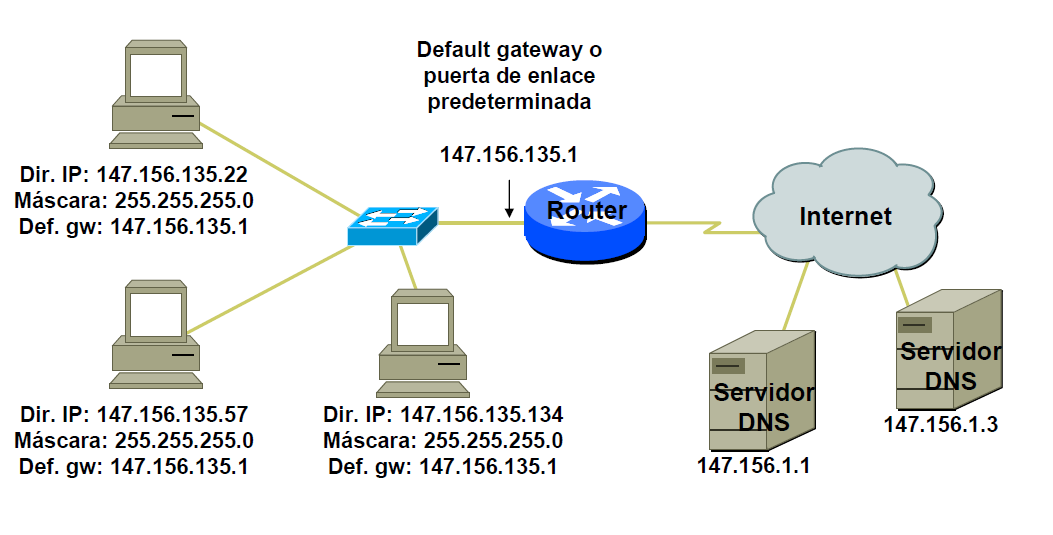
\includegraphics[width=0.8\textwidth]{graficos/RED_LOCAL.png}
     \label{fig:RED_LOCAL} 
	\end{center}    
    \caption{Representaci\'on visual de una red local.}  
    
\end{figure}
\vspace{1cm}

En el ejemplo de la figura anterior puede observarse que los hosts utilizan la subm\'ascara de red 255.255.255.0, esto implica que cualquier direcci\'on IP de la pinta 147.156.135.X debe tratarse como una direcci\'on dentro de la red local. En caso de una IP que no se corresponda con esta m\'ascara se espec\'ifica el gateway por defecto 147.156.135.1. \\\

Algunos ejemplos,
\begin{itemize}
\item El host 147.156.135.22 necesita resolver la IP 147.156.135.57. Por la m\'ascara de red sabe que la direcci\'on se encuentra en la red local y env\'ia un paquete ARP \textit{who-has} para resolver su mac address. El paquete es recibido por todos los hosts de la red pero solo el host 147.156.135.57 responde con un paquete ARP \textit{is-at} env\'iando su mac address. Una vez recibido este paquete ahora el host 147.156.135.22 tiene resuelta la mac address para poder comunicarse localmente.

\item El host 147.156.135.22 necesita resolver la IP 147.156.135.101. Por la m\'ascara de red sabe que la direcci\'on se encuentra en la red local y env\'ia un paquete ARP \textit{who-has} para resolver su mac address. El paquete es recibido por todos los hosts de la red pero no existe el host 147.156.135.101. El host 147.156.135.22 intepretara la falta de respuesta como que el nodo 147.156.135.101 es inexistente en la red o se encuentra ca\'ido.

\item El host 147.156.135.22 necesita resolver la IP 74.125.236.34. Por la mascara de red sabe que la direcci\'on no se encuentra en la red local y resuelve utilizar el gateway por defecto 147.156.135.1. Ahora el paquete es recibido por todos los host de la red pero solo el host 147.156.135.57 responde con un paquete ARP \textit{is-at} env\'iando su mac address. Una vez recibido este paquete el host 147.156.135.22 tiene resuelta la mac address para poder comunicarse localmente con el router. El router se encarga de enviar los paquetes enviados hac\'ia la direcci\'on 74.125.236.34 por la interfaz correspondiente. \\\


\end{itemize}


\begin{figure}[H]
	\begin{center}
    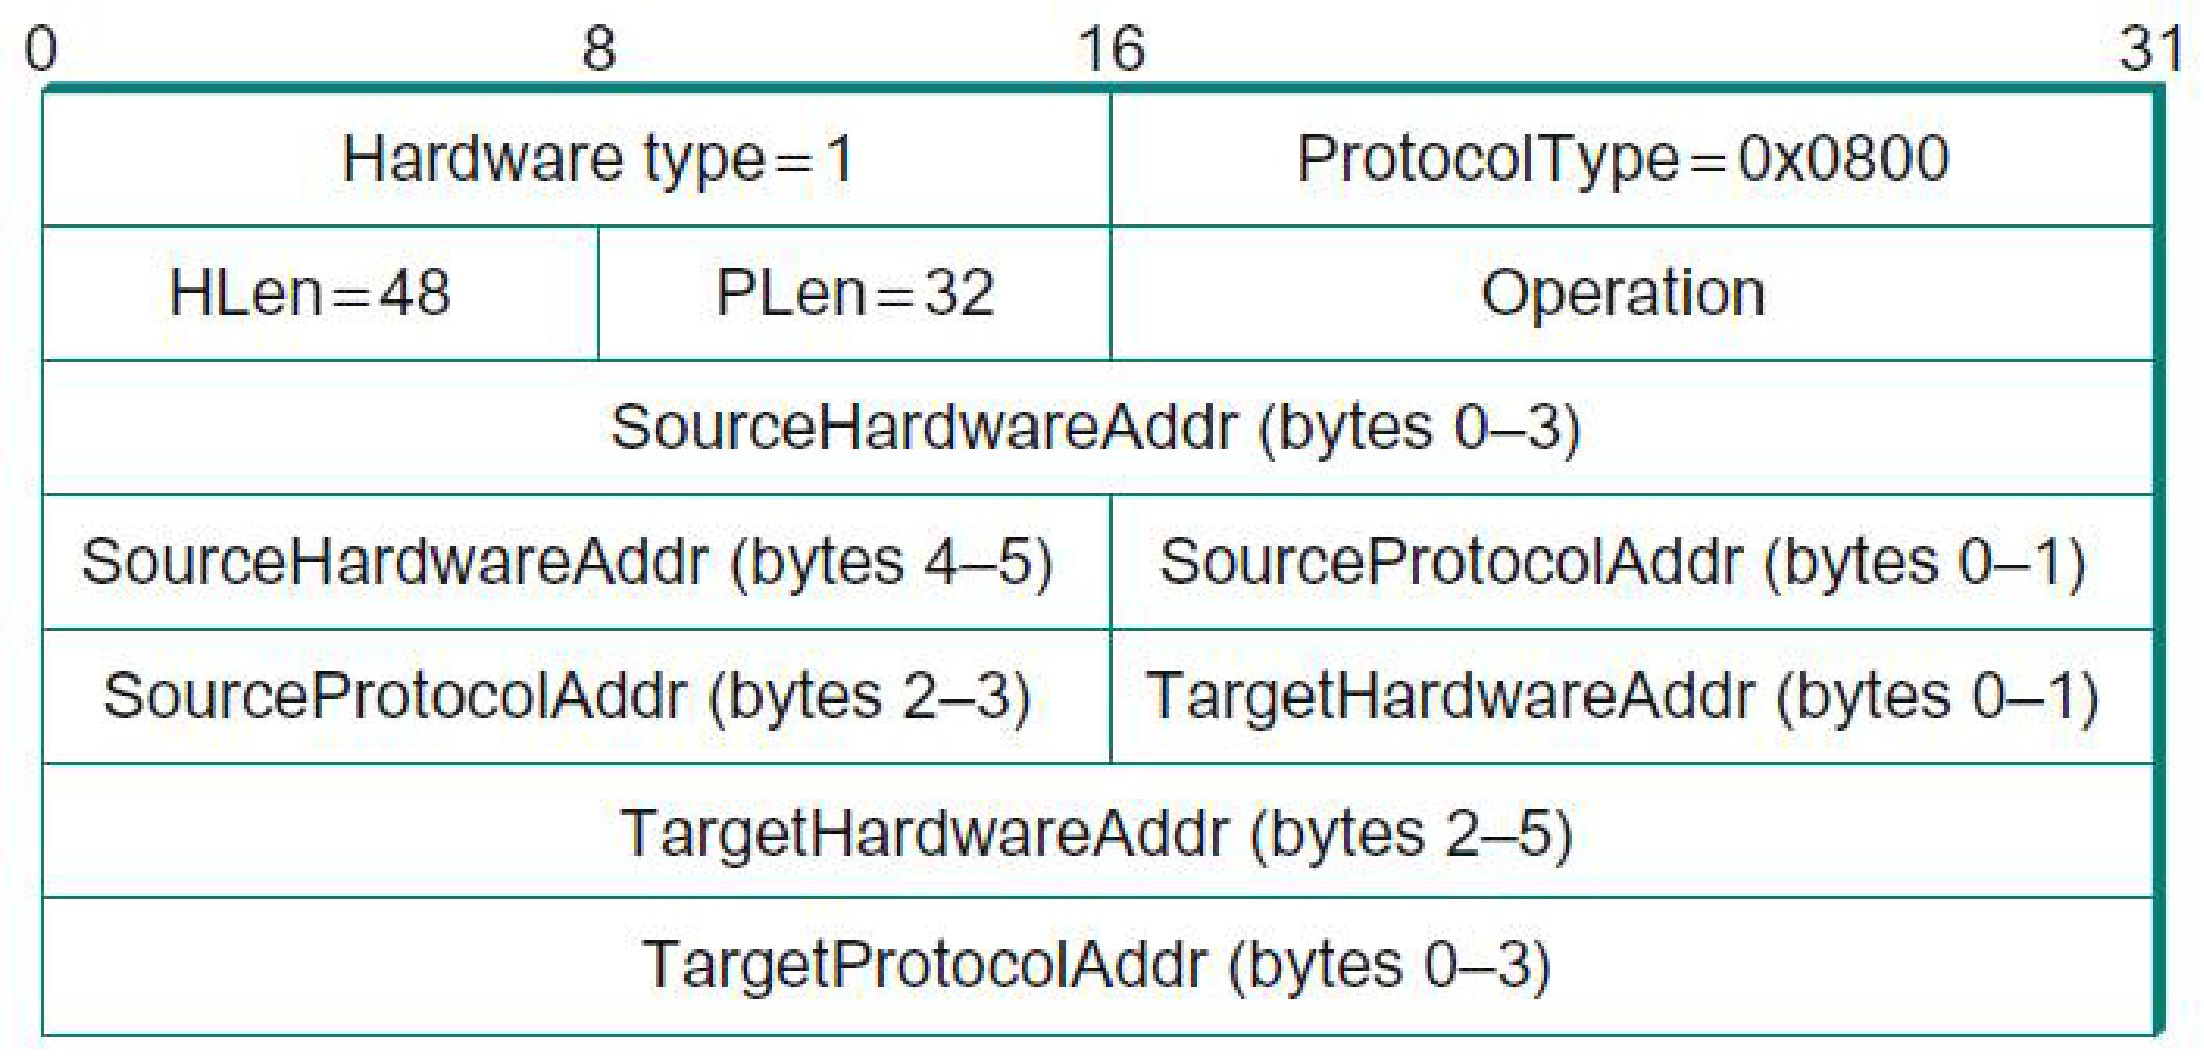
\includegraphics[width=0.8\textwidth]{graficos/ARP_PACKET.png}
	\end{center}    
    \caption{Estructura del paquete ARP.}
\label{fig:ARP_PACKET} 
\end{figure}

\vspace{1cm}

Campos del paquete \textit{ARP}
\begin{itemize}
\item Hardware type (HTYPE) \\
Este campo espec\'ifica el tipo de hardware utilizado para la transmisi\'on local del mensaje ARP. 	Ejemplos: 1 Ethernet, 6 IEEE 802 Networks, 7 ARCNET, 15 Frame relay, etc. \\\

\item Protocol type (PTYPE) \\
	Este campo complementa el HTYPE espec\'ificando el tipo de direcciones de capa 3 usadas en el mensaje. Ejemplos: 0x0800 IPV4, 0x0842 Wake-On-Lan, 0x809B AppleTalk, etc. Estos c\'odigos coinciden con los c\'odigos EtherType (c\'odigos utilizados para indicar que tipo de protocolo se encuentra encapsulado en el payload de un frame ethernet). \\\
	
\item Hardware length (HLEN)\\
Espec\'ifica cuan largas son las direcciones del hardware en el mensaje. Ejemplos: Para Ethernet u otras redes que utilicen IEEE 802 MAC addresses el valor es 6. \\\

\item Protocol length (PLEN) \\
Espec\'ifica cuan largas son las direcciones de capa 3 utilizadas en el mensaje. Ejemplos: Para IPv4 el valor es por supuesto 4. \\\

\item Operation  \\
Espec\'ifica el tipo de mensaje ARP que se esta enviando. Ejemplo: 1 para request, 2 para reply (t\'ipicamente se utilizan solo estos valores). \\\
  
\item  Sender hardware address (SHA) \\
   MAC address de quien env\'ia el mensaje. En un request ARP el campo \'indica la direcci\'on del host que env\'ia el request. En un reply ARP el campo es utilizado para indicar la direcci\'on del host que el request estaba buscando (no necesariamente la direcci\'on que responde al pedido). Notar que los switches no utilizan este campo para aprender la MAC address. \\\
   
   
\item Sender protocol address (SPA) \\
    Direcci\'on de red del host que origina el mensaje. \\\
    
\item Target hardware address (THA) \\
    En un request ARP este campo es ignorando. En un reply ARP este campo es usado para indicar la direcci\'on del host que origin\'o el request (obteniendose del SHA).\\\

\item Target protocol address (TPA) \\
   	Direcci\'on de red del receptor esperado. \\\
\end{itemize}




\subsection{Informaci\'on y entrop\'ia}
En el contexto de la teor\'ia de la informaci\'on la entrop\'ia, tambi\'en llamada entrop\'ia de la informaci\'on y entrop\'ia de Shannon (en honor a Claude E. Shannon), mide la incertidumbre de una fuente de informaci\'on. Intuitivamente mide la cantidad de ''desorden'' o ''aleatoriedad'' de una fuente de informaci\'on. A mayor entrop\'ia de una fuente de informaci\'on menos predicciones pueden hacerse sobre datos que se obtengan de la fuente. En el caso contrario cuando la entrop\'ia es nula puede predecirse con exactitud la informaci\'on contenida en la fuente. \\\

La entrop\'ia tambien puede interpretarse como la media de informaci\'on contenida por los s\'imbolos de la fuente. Si suponemos como ejemplo una fuente donde los s\'imbolos son palabras y conocemos de antemano que hay palabras con mucha probabilidad de aparecer en un mensaje (una cadena de s\'imbolos) en comparaci\'on al resto, al mismo tiempo sabemos que aportan poca ``informaci\'on'' a lo que el mensaje quiere expresar y que se requeriran de las palabras con menos probabilidad para diferenciarlo del resto. De esta manera podemos intuir que los s\'imbolos con mayor probabilidad son los que menos informaci\'on aportan. \\\

El concepto de entrop\'ia se concibe como una medida del desorden o la peculiaridad de ciertas combinaciones. La entrop\'ia puede ser considerada como una m\'etrica de la incertidumbre alrededor de un proceso.\\\

Shannon ofrece una definici\'on de entrop\'ia que satisface las nociones:
\begin{itemize}
\item La medida de información debe ser proporcional (lineal continua). Es decir, el cambio pequeño en una de las probabilidades de aparición de uno de los elementos de la señal debe cambiar poco la entropía.

\item Si todos los elementos de la señal son equiprobables a la hora de aparecer, entonces la entropía será máxima. \\\
\end{itemize}

\subsubsection{Definici\'on formal}
Sea $S$ una fuente de informaci\'on emitiendo s\'imbolos que pertenecen a un alfabeto que podemos suponer finito $S = \{s_{1}, \ldots, s_{n}\}$. Los s\'imbolos emitidos se rigen por una ley fija de probabilidad. Como abuso notacional nos referiremos a la fuente misma como $S$. Tal fuente de informaci\'on se conoce como fuente de informaci\'on nula y la probabilidad de cada s\'imbolo queda definida como $P(s_{1}), \ldots, P(s_{n})$. \\\

La informaci\'on aportada por un s\'imbolo $s_{i}$ en $bits$ quedara determinada por:
\begin{gather*}
I(s_{i}) = log_{2}[1 / P(s_{i})] = - log_{2}P(s_{i}) = - log_{2}p_{s_{i}}
\end{gather*}
\vspace{1cm}

De esta manera la media de informaci\'on de la fuente queda determinada por:
\begin{gather*}
\sum_{s \in S}^{} P(s)I(s) \text{ bits} = - \sum_{i = 0}^{n} p_{s_{i}}log_{2}p_{s_{i}}  \text{ bits}
\end{gather*}
\vspace{1cm}

Llamaremos a este valor la entrop\'ia de la fuente $S$ y lo escribiremos:
\begin{gather*}
H(S) = - \sum_{i = 0}^{n} p_{s_{i}}log_{2}p_{s_{i}}  \text{ bits}
\end{gather*}
\vspace{1cm}

La entrop\'ia cumple que:
\begin{itemize}
\item La entropía $H(S)$ es no negativa.
\item La entrop\'ia $H(S)$ esta acotada superiormente.
\item La entrop\'ia $H(S)$ es m\'axima $\iff$ todos los s\'imbolos de la fuente son equiprobables. 
\end{itemize}
\vspace{1cm}

La entrop\'ia $H(S)$ de una fuente de s\'imbolos $S$ tiene las siguientes interpretaciones:
\begin{itemize}
\item Es el valor medio ponderado de la cantidad de informaci\'on del conjunto de mensajes posibles
\item Una medida de la incertidumbre promedio (grado de incerteza) acerca de una variable aleatoria
\item La cantidad de informaci\'on obtenida al observar la aparici\'on de
cada nuevo s\'imbolo.
\end{itemize}
\vspace{1cm}